\documentclass{beamer}
\usepackage[utf8]{inputenc}
\usepackage{amsfonts,amsmath,oldgerm}
\usetheme{sintef}

\usefonttheme[onlymath]{serif}

\titlebackground*{assets/background}

\newcommand{\hrefcol}[2]{\textcolor{cyan}{\href{#1}{#2}}}

\title{Riconoscimento di dispositivi di
protezione individuale in ambito
industriale tramite infrastruttura
cloud}
%\subtitle{Sottotitolo della Tesi (se necessario)}
\course{Corso di Laurea Magistrale in Ingegneria Informatica}
\author{\href{mailto:rei.zoto@studenti.polito.it}{Rei Zoto}}
\IDnumber{Matricola: 258017}

\begin{document}
\maketitle

\section{Introduzione}

\begin{frame}{Infortuni sul Lavoro}
\begin{itemize}
    \item Problemi
    	\begin{itemize}
    		\item costi diretti
    		\item costi indiretti
    		\item impatto sulla società
    	\end{itemize}	
    \item Soluzioni
    \begin{itemize}
    	\item Prevenzione: valutazione dei rischi, idoneità del lavoratore, formazione
    	\item Dispositivi di sicurezza individuale (DPI)
    	\item Sistemi automatici al posto di controlli manuali
    \end{itemize}
\end{itemize}
\end{frame}

\begin{frame}{INAIL: Statistiche sugli infortuni}
  \begin{itemize}
  		\item Totale infortuni nella manifattura anno 2022: 13,9\%
  \end{itemize}  	  
  \begin{columns}
    % Prima colonna
    \begin{column}{0.4\textwidth}
      \centering
      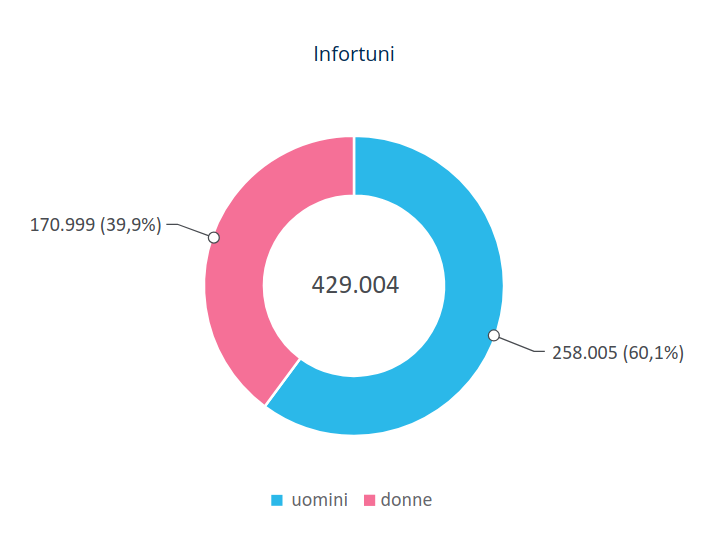
\includegraphics[width=\textwidth]{images/totaleinfortuni.png}
      \vspace{2mm}
      \small{Totale infortuni divisi per genere}
    \end{column}

    % Seconda colonna
    \begin{column}{0.3\textwidth}
      \centering
      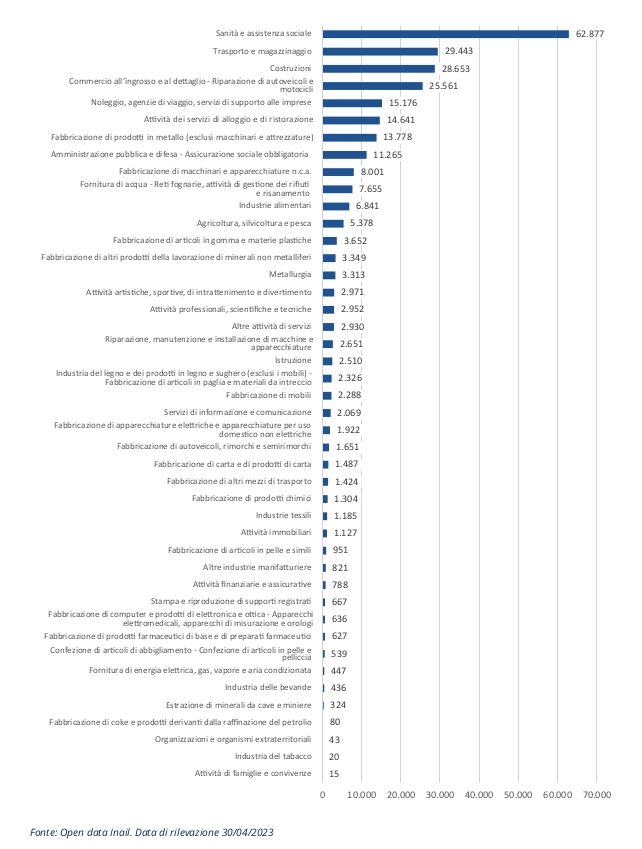
\includegraphics[width=\textwidth]{images/infortuni_industria_e_servizi.png}
      \vspace{2mm}
      \small{Infortuni per categoria}
    \end{column}
  \end{columns}
\end{frame}











\begin{frame}{OSHA-EU: Impatto sulla produttività nazionale}
%  \begin{itemize}
%  	\item DALY: stima anni di vita persi per infortuni e malattie
%	\item VSLY: metodologia che associa agli anni di vita un valore monetario

%  \end{itemize}
  \begin{columns}  
    % Prima colonna
    \begin{column}{0.5\textwidth}
      \centering
      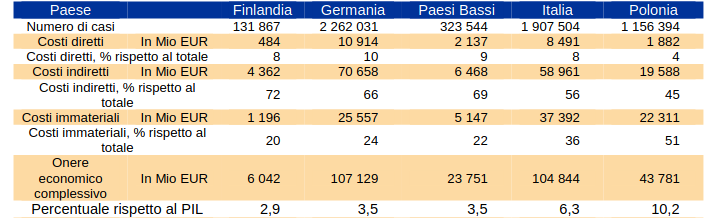
\includegraphics[width=\textwidth]{images/onere_infortuni_ba.png}
      \vspace{2mm}
      \small{Approccio bottom-up}
    \end{column}

    % Seconda colonna
    \begin{column}{0.5\textwidth}
      \centering
      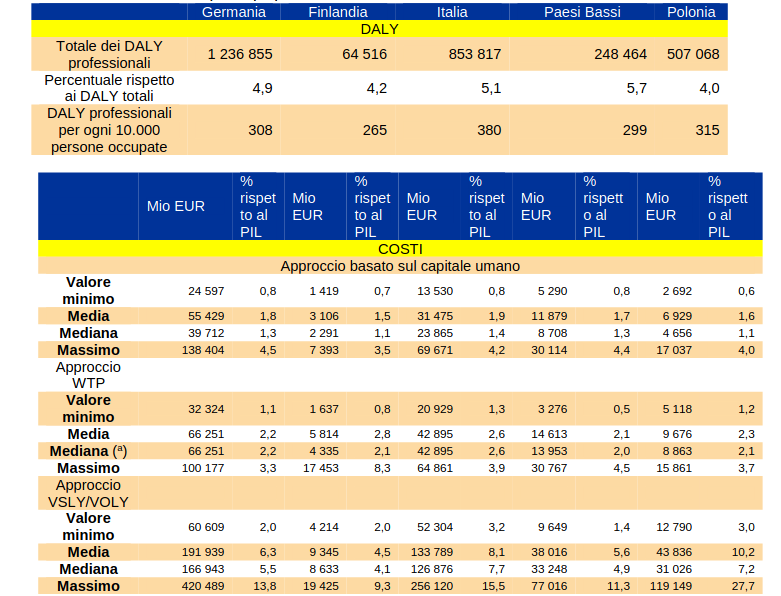
\includegraphics[width=\textwidth]{images/onere_infortuni_td.png}
      \vspace{2mm}
      \small{Approccio top-down}
    \end{column}
  \end{columns}
\end{frame}

\begin{frame}{Obiettivi e Motivazioni}
\textbf{Scopo del lavoro}:
\begin{itemize}
	\item Implementazione di un sistema integrato con il cloud per la rilevazione di dispositivi di sicurezza    
    \item Modelli pronti all'uso forniti da provider cloud
    
\end{itemize}

\textbf{Motivazioni personali}:
\begin{itemize}
    \item Interesse sistemi IoT e deep learning
    \item Scelta della tesi durante lo studio di sistemi operativi, virtualizzazione ed estensione dei concetti al cloud.
\end{itemize}
\end{frame}







\section{Panoramica}

\begin{frame}{Fattori abilitanti}
\begin{itemize}
	\item Quantità di dati disponibili provenienti dai dispositivi connessi alla rete
	\item Avanzamenti deep learning
	\item Cloud computing: potenza di calcolo ed integrazione di modelli e dati nell'ecosistema industriale
	\item Investimenti (cita i ritorni economici previsti dallo studio, ma anche l'hype attuale su ai)
\end{itemize}
\end{frame}

%prova a rendere più densa questa slide
\begin{frame}{Computer Vision}
	\begin{itemize}
	\item Utilizzo modelli di deep learning per task di computer vision
			%classificazione
			%object detection
			%image segmentation
			%image generation, encoding
	\item Dominio di applicazione: object detection
	\item Modello utilizzato: Amazon Rekognition %descrivi come funziona
	\item[] % Elemento senza bullet
    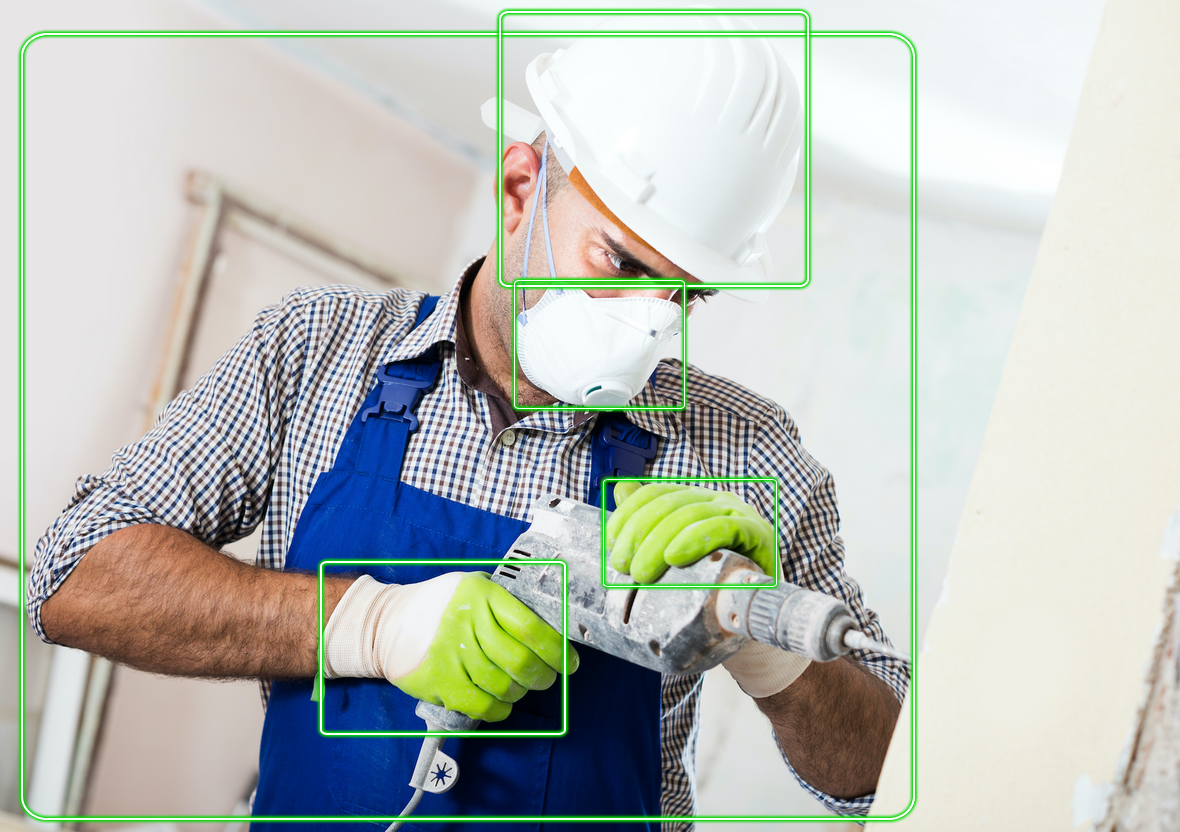
\includegraphics[width=0.3\textwidth]{images/worker-with-bb.png}
	\end{itemize}
\end{frame}

\begin{frame}{Lavori Correlati}
  \begin{columns}
    % Prima colonna
    \begin{column}{0.5\textwidth}
      \centering
      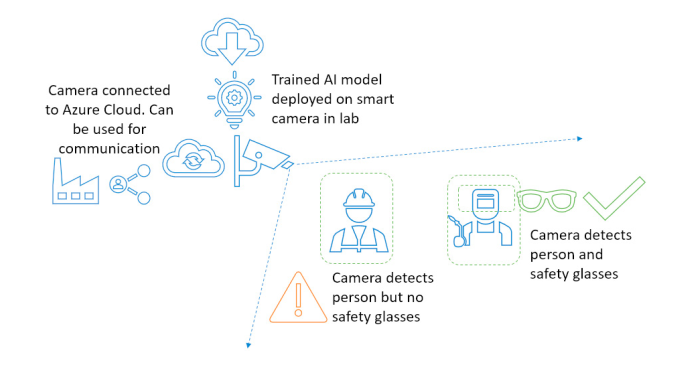
\includegraphics[width=\textwidth]{images/relw1-system.png}
      \tiny B. Balakreshnan and Others, “Ppe compliance detection using artificial
intelligence in learning factories”
    \end{column}

    % Seconda colonna
    \begin{column}{0.5\textwidth}
      \begin{figure}
      \centering
      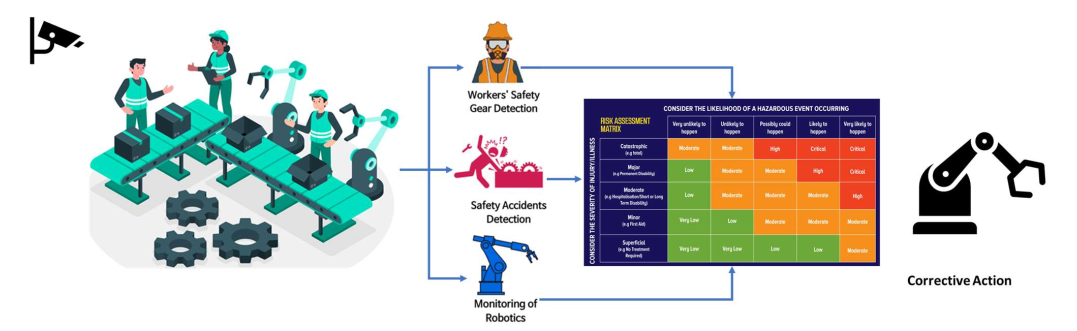
\includegraphics[width=\textwidth]{images/safety-system.png}
      \caption{\tiny {I. Yousif and Others, “Safety 4.0: Harnessing computer vision for
advanced industrial protection”}}
	\end{figure} 
    \end{column}
  \end{columns}
\end{frame}

%\begin{frame}{Lavori Simili (cont.)}
%  \begin{columns}
    % Prima colonna
%    \begin{column}{0.4\textwidth}
%      \centering
%      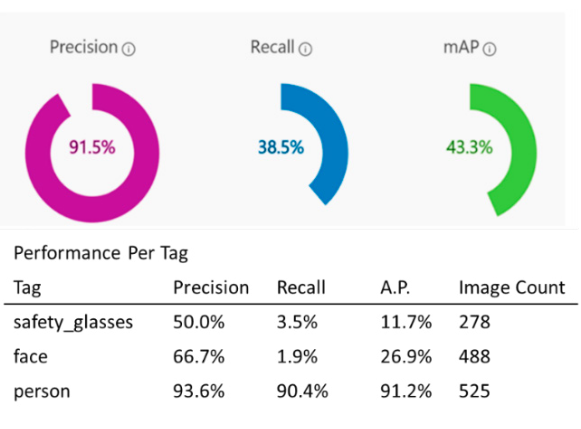
\includegraphics[width=\textwidth]{images/relw1.png}
%      \vspace{2mm}
%      \small{1) Metriche sulle classi maschera protettiva, volti e persone}
%    \end{column}

    % Seconda colonna
%    \begin{column}{0.4\textwidth}
%      \centering
%      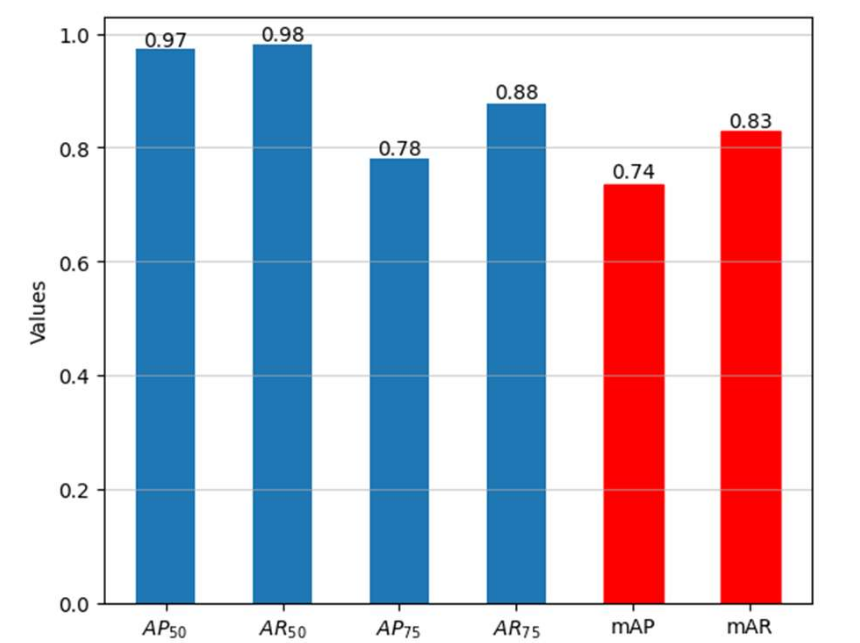
\includegraphics[width=\textwidth]{images/safety-system-results.png}
%      \vspace{2mm}
%      \small{2) Mean Average Precision sulle classi casco e giubotto protettivo}
%    \end{column}
%  \end{columns}
%\end{frame}


\begin{frame}{Soluzione}

\begin{itemize}
    \item Risposta al problema con un sistema near real-time.
    \item Posizionamento della soluzione rispetto agli approcci precedenti
\end{itemize}

\textbf{Motivazioni}:
\begin{itemize}
    \item Mancanza di benchmark specifici per dispositivi di sicurezza.
    \item L'approccio near real-time è conservativo a causa di:
    \begin{itemize}
        \item Tempi di risposta del modello non veloci (servizio pensato per tutti gli utenti AWS, tipicamente 5 fps).
        \item Latenza intrinseca per la comunicazione con il cloud e problemi di connettività.
    \end{itemize}
\end{itemize}
\end{frame}

\begin{frame}{Tecnologie Utilizzate}
    \centering
    \begin{tabular}{ccc}
        % Prima Riga: Docker, AWS, Apache Flink
        
\includegraphics[width=0.2\textwidth]{images/docker_logo.png} & 
        
\includegraphics[width=0.2\textwidth]{images/aws_logo.png} & 
        
\includegraphics[width=0.2\textwidth]{images/apache_flink_logo.jpeg} \\
         	& 	 & Apache Flink \\
        \vspace{0.5cm} \\ % Spazio aggiuntivo tra le righe
        % Seconda Riga: MQTT, RTSP, Publish/Subscribe
        
\includegraphics[width=0.2\textwidth]{images/mqtt_logo.png} & 
        
\includegraphics[width=0.2\textwidth]{images/rtsp_logo.png} \\ 
    \end{tabular}
    \footlinecolor{sintefyellow}
\end{frame}

%vedi se aggiungere, forse too much ma sarebbe utile per la comprensione
%\begin{frame}{Servizi utilizzati}
%\end{frame}
\section{Implementazione}
\begin{frame}{Use Case}
\begin{columns}
\begin{column}{0.5\textwidth}
\footnotesize
\begin{itemize}
	\item Scenario	
\begin{itemize}
\footnotesize
	\item Uno o più operatori entrano all’interno di una certa area di sicurezza e si trovano in prossimità di un macchinario attivo
	\item Una telecamera sul soffitto ed una frontale monitorano l’area di sicurezza
	\item La zona è definita da un insieme di ancore dotate di sensori che rilevano i tag indossati dai lavoratori. 
\end{itemize}
	\item Il sistema genera allarme e spegne il macchinario	
\begin{itemize}
\footnotesize
	\item Almeno uno degli operatori non possiede i dispositivi di sicurezza
	\item Almeno uno degli operatori non è abilitato ad agire sulla macchina
\end{itemize}
\end{itemize}
\end{column}
\begin{column}{0.5\textwidth}
	\begin{figure}	
	\centering
    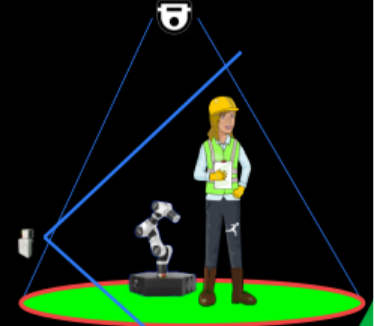
\includegraphics[width=0.7\textwidth]{images/use-case.png}
    \end{figure}
\end{column}
\end{columns}
\end{frame}

\begin{frame}{Architettura}
\begin{figure}
    \centering
    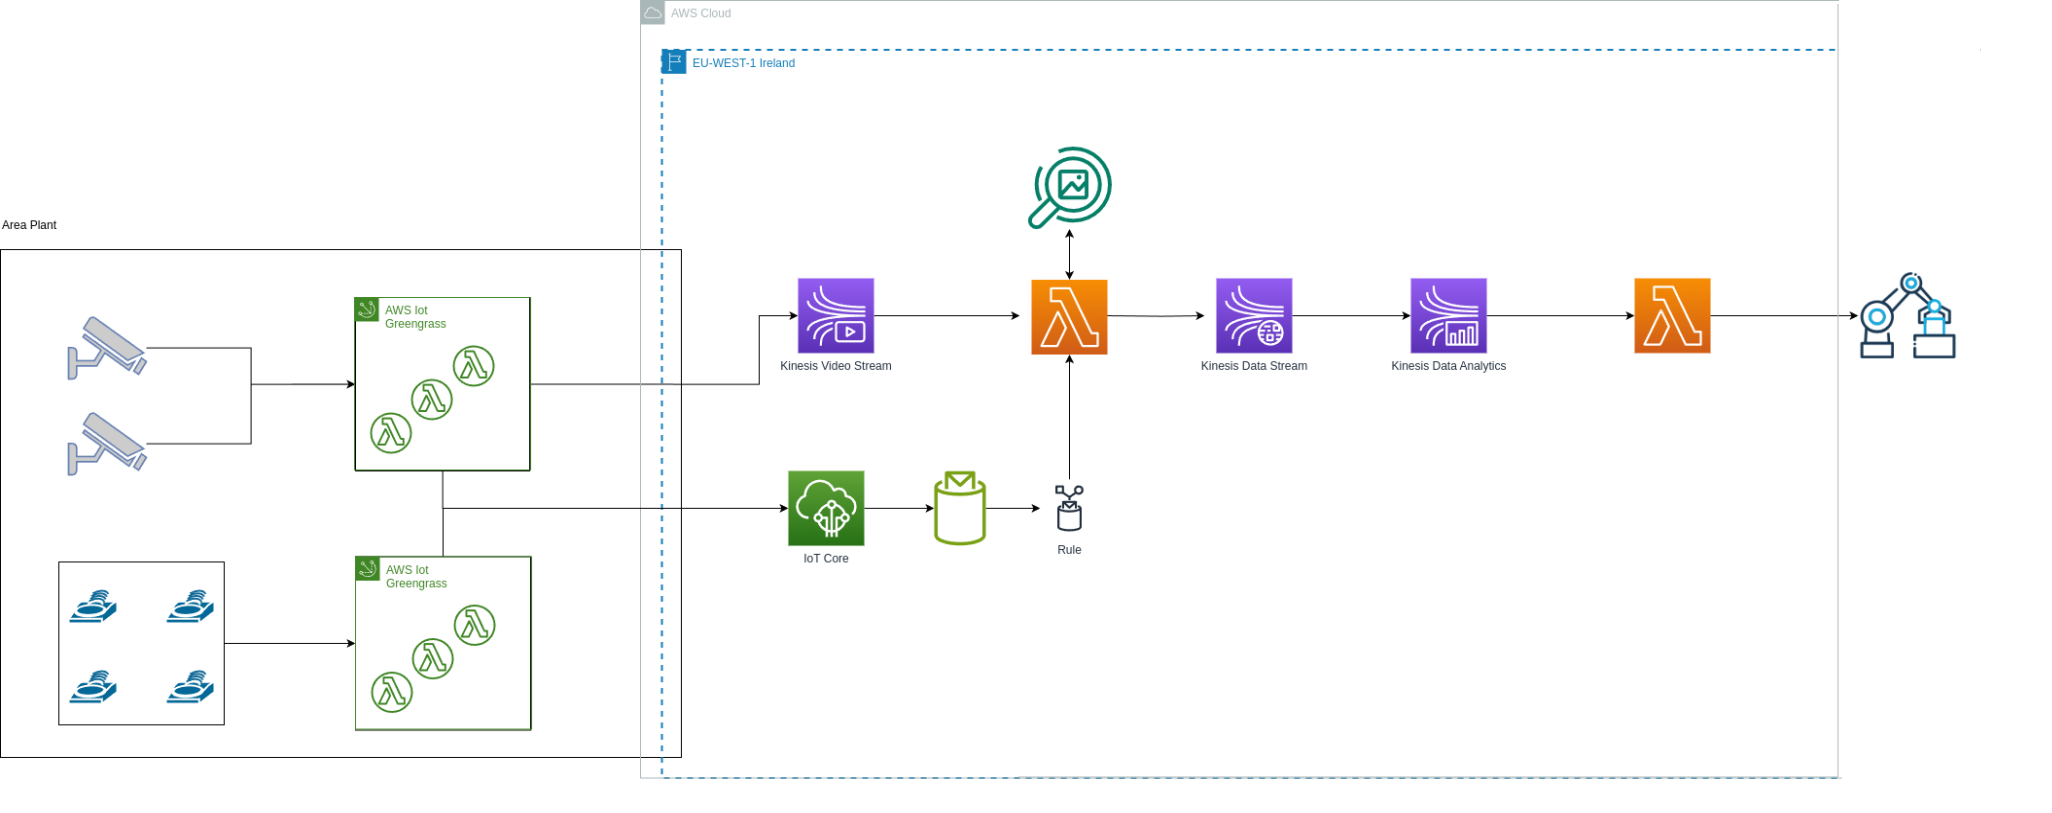
\includegraphics[width=0.9\textwidth]{images/architettura.png}
%    \caption{Diagramma dell'Architettura Generale}
\end{figure}
\end{frame}

\begin{frame}{Ingestion e Preprocessing}
\begin{figure}
    \centering
    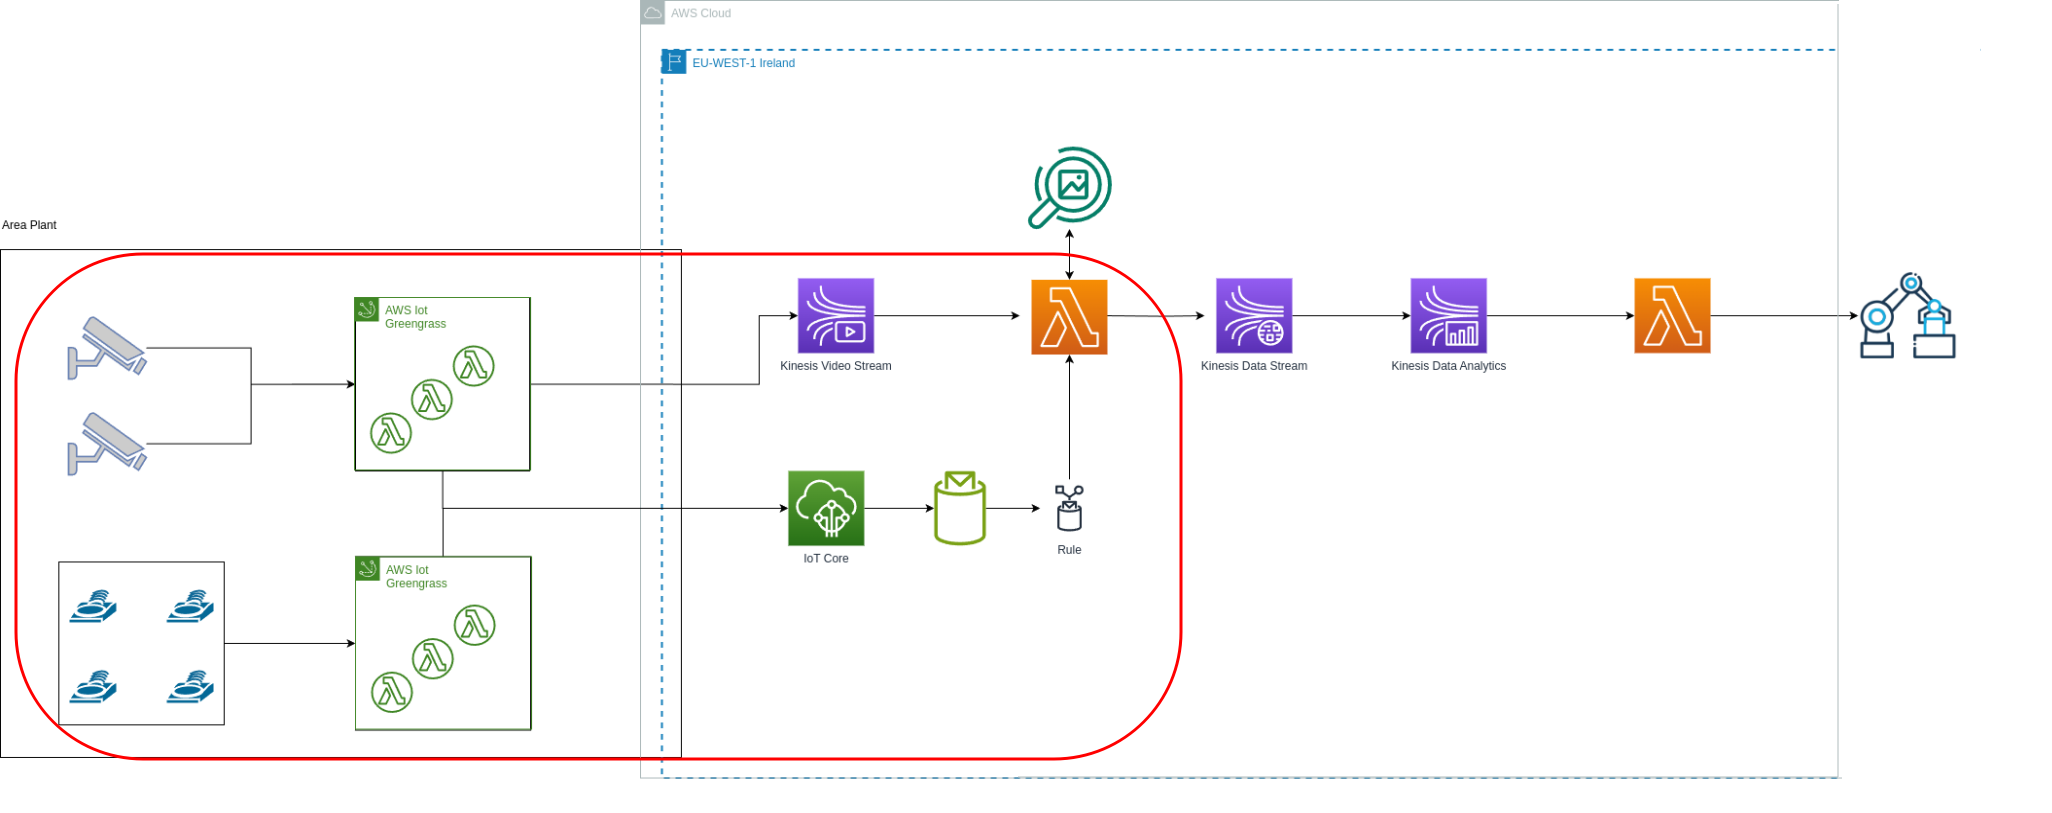
\includegraphics[width=0.9\textwidth]{images/sottosistema-ingestion.png}
%    \caption{Diagramma dell'Architettura Generale}
\end{figure}

\end{frame}

\begin{frame}{Big Data Processing}
\begin{figure}
    \centering
    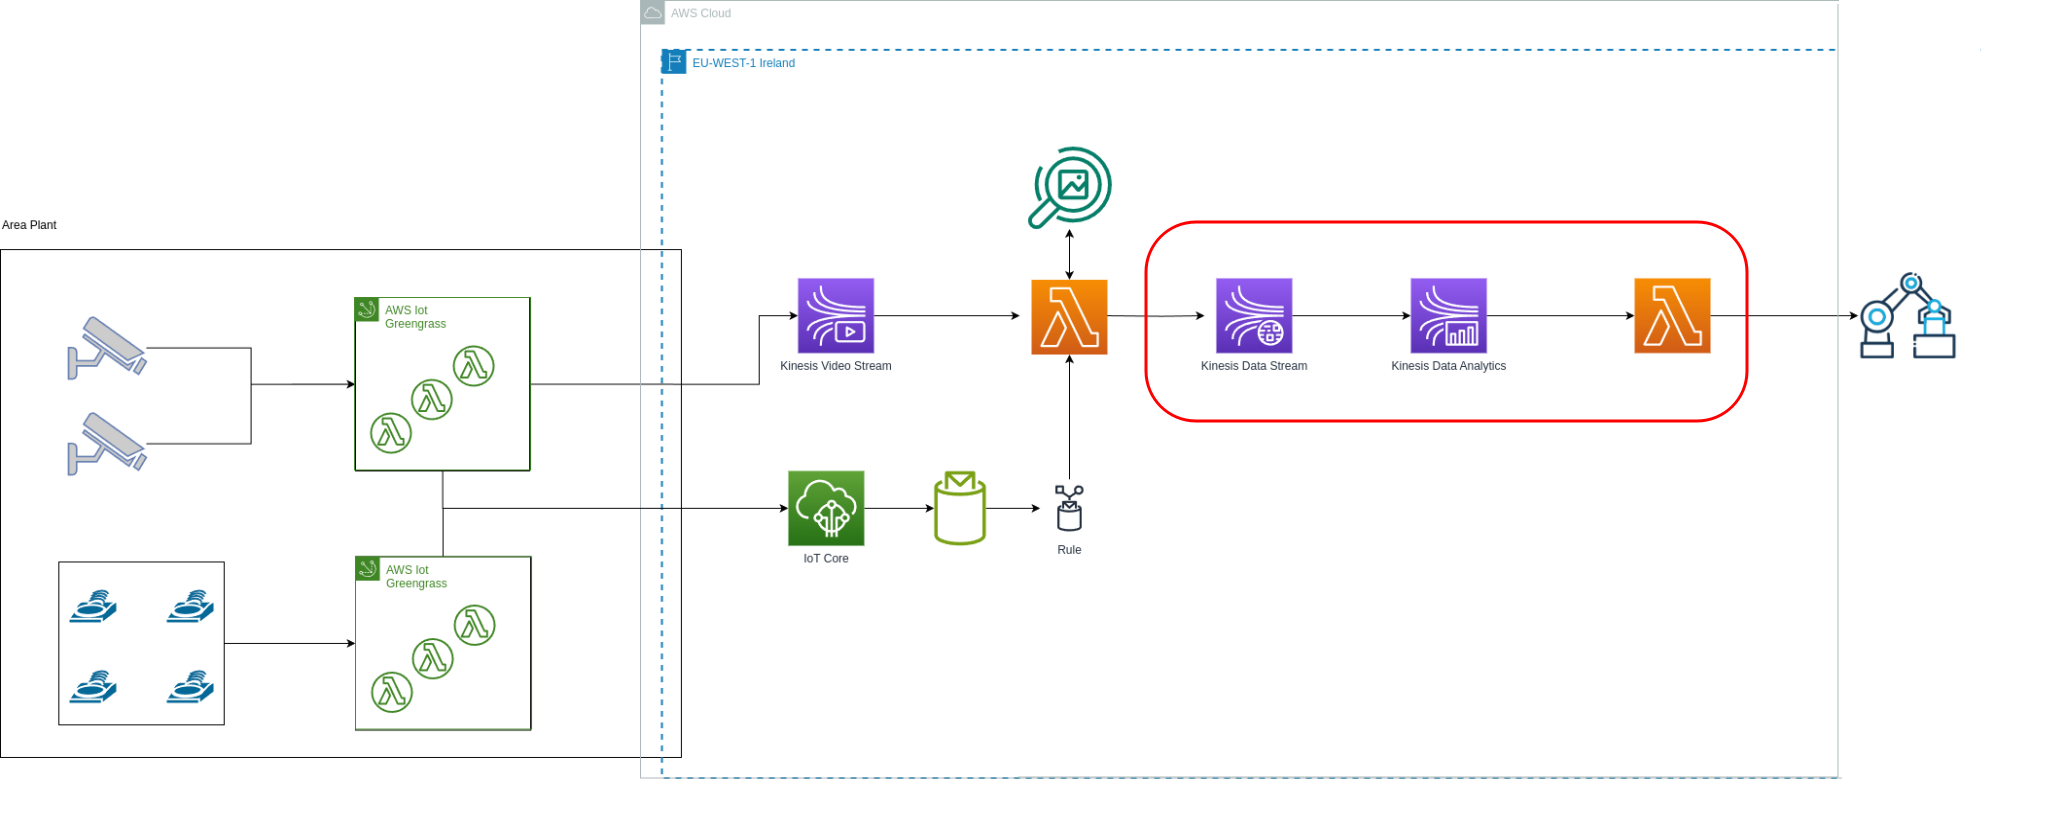
\includegraphics[width=0.9\textwidth]{images/processing-subsystem.png}
%    \caption{Diagramma dell'Architettura Generale}
\end{figure}

\end{frame}


\section{Risultati}

\begin{frame}{Test}
\textbf{Funzionalità Raggiunte}:
\begin{itemize}
    \item Rilevazioni near real-time nei 5 test case
    \item Dettagli funzionali e metriche
\end{itemize}
\end{frame}

\begin{frame}{Metriche}
\textbf{Funzionalità Raggiunte}:
\begin{itemize}
    \item Rilevazioni near real-time nei 5 use case.
    \item Dettagli funzionali e metriche.
\end{itemize}
\end{frame}

\begin{frame}{Limitazioni}
\begin{itemize}
    \item Discussione delle limitazioni dell'approccio.
    \item L'azienda ha deciso di passare a una soluzione edge su mio consiglio, estensione di questo progetto.
    \item Consapevolezza delle differenze rispetto ai lavori accademici più complessi.
\end{itemize}
\end{frame}

\section{Conclusioni}

\begin{frame}{Conclusioni e Sviluppi futuri}
\begin{itemize}
    \item Riepilogo dei punti chiave.
    \item Potenziali miglioramenti ed estensioni future.
\end{itemize}
\end{frame}

\section*{Domande}

\backmatter
\end{document}
